\documentclass[tikz,border=3pt]{standalone}

% TikZ + PGFPlots
\usepackage{tikz}
\usepackage{tikzfmv}
\usepackage{pgfplots}
\pgfplotsset{compat=1.18}

\usetikzlibrary{shapes.misc}
\usetikzlibrary{arrows.meta,
                calc,
                positioning,
                intersections,
                decorations.pathreplacing,
                decorations.markings,
                patterns,angles,quotes}

\usepgfplotslibrary{fillbetween,groupplots}

\definecolor{headingscolor}{RGB}{0,90,150}

% Styles généraux
\tikzset{
  >=Stealth,
  axis/.style={thick,->},
  signal/.style={thick},
  construction/.style={dashed,gray},
  block/.style={draw,rectangle,minimum height=2em,minimum width=3em}
}

% Configuration par défaut des axes PGFPlots
\pgfplotsset{
  every axis/.style={
    thick,
    grid=both,
    grid style={gray!30},
    major grid style={gray!50}
  }
}

% Styles spécifiques Bode (adaptés à ton livre)
\pgfplotsset{
  bode magnitude/.style={xmode=log,xlabel={$\omega$},ylabel={Gain (dB)}},
  bode phase/.style={xmode=log,xlabel={$\omega$},ylabel={Phase (deg)}}
}



\begin{document}

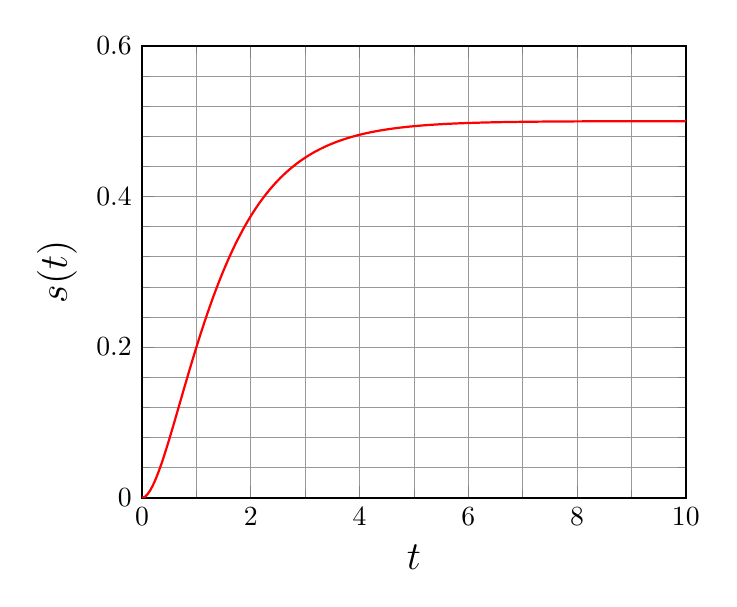
\begin{tikzpicture}
    \begin{axis}[
        width=0.7\linewidth,
        legend style={draw=none},
        legend pos=south west,
        axis line style = thick,
        xmin=0,
        xmax=10,
        ymin=0,
        ymax=0.6,
        xlabel={$t$},
        ylabel={$s(t)$},
        label style={font=\Large},
        minor y tick num=4,
        minor x tick num=1,
        grid=both,
        grid style={line width=.2pt, draw=gray!80},
        major grid style={line width=.2pt,draw=gray!80},
    ]
        \addplot[thick,color=red,domain=0:10,samples=201]
        {0.5*(1-2*exp(-x)+exp(-2*x))};
    \end{axis}
\end{tikzpicture}

\end{document}
